 \documentclass[12pt,answers]{exam}
%\documentclass[12pt]{exam}
\usepackage{amsmath}
\usepackage{listings}
\usepackage{graphicx}
\usepackage{semantic}

\newcommand{\itm}[1]{\ensuremath{\mathit{#1}}}
\newcommand{\key}[1]{\texttt{#1}}

\lstdefinestyle{basic}{showstringspaces=false,columns=fullflexible,language=Python,
escapechar=@,xleftmargin=1pc,%
%basicstyle=\small\bfseries\itshape,%
%keywordstyle=\underbar,
mathescape=false,%
escapechar=|,%
lineskip=-1pt,%
keepspaces=true,%
%basicstyle=\small\sffamily,%
basicstyle=\footnotesize\ttfamily,%
commentstyle=\mdseries\rmfamily,%
morekeywords={class,object,with,fun,new,end,int,bool,string},%
deletekeywords={error,apply,values,and,equal,eq},%
%moredelim=**[is][\color{red}]{`}{`}
}
\lstset{style=basic}

\firstpageheader{\bf\large Compiler Construction\\ Professor Jeremy Siek\\[1ex]}%
{}%
{\bf Midterm Exam \\March 9, 2016\\[1ex]Name:\enspace\hbox to 2in{\hrulefill}}
\firstpageheadrule

\runningheader{Compiler Construction\\[1ex]}%
{Midterm Exam \\ }%
{March 9, 2016\\[1ex] Name:\enspace\hbox to 2in{\hrulefill}}

\runningfooter{}{Page \thepage\ of \numpages}{}
\runningheadrule
\runningfootrule

\extraheadheight{.75in}
\extrafootheight{-.5in}

\addpoints
\boxedpoints

\begin{document}

\vspace{20pt}

\begin{center} 
This exam has \numquestions\ questions, for a total of \numpoints\ 
points. 
\end{center} 

\begin{questions}

% topics:
%   Integer arithmetic and let
% *   flatten
%     instruction selection (x86 knowledge)
%     stack alocation
% *   patch-instructions

\question[10] Compile the following Racket program to an equivalent
program in the $C_0$ language defined in Figure~\ref{fig:c0-syntax}.
\begin{lstlisting}
  (- (+ (read) 10))
\end{lstlisting}

\begin{figure}[h]
\centering
\fbox{
\begin{minipage}{0.65\textwidth}
\[
\begin{array}{lcl}
\itm{arg} &::=& \itm{int} \mid \itm{var} \\
\itm{exp} &::=& \itm{arg} \mid (\key{read}) \mid (\key{-}\;\itm{arg}) \mid (\key{+} \; \itm{arg}\;\itm{arg})\\
\itm{stmt} &::=& (\key{assign}~\itm{var}~\itm{exp}) \mid (\key{return}~\itm{arg}) \\
C_0 & ::= & (\key{program}\;(\itm{var}^{*})\;\itm{stmt}^{+})
\end{array}
\]
\end{minipage}
}
\caption{The $C_0$ intermediate language.}
\label{fig:c0-syntax}
\end{figure}


\begin{solution}[1in]
\begin{lstlisting}
(program (t1 t2 t3)
  (assign t1 (read))
  (assign t2 (+ t1 10))
  (assign t3 (- t2))
  (return t3))
\end{lstlisting}
\end{solution}

\question[10] Given the following psuedo-x86 program, compile it to an
equivalent x86 program, using stack locations (and not registers) for
the variables \texttt{x} and \texttt{t}.
\begin{lstlisting}
(program (x t)
  (callq read_int)
  (movq (reg rax) (var x))
  (movq (var x) (var t))
  (addq (var x) (var t))
  (movq (var t) (reg rax)))
\end{lstlisting}

\begin{solution}[3in]
\begin{lstlisting}
	.globl main
main:
	pushq	%rbp
	movq	%rsp, %rbp
	subq	$16, %rsp

	callq	read_int
	movq	%rax, -8(%rbp)
	movq	-8(%rbp), %rax
	movq	%rax, -16(%rbp)
	movq	-8(%rbp), %rax
	addq	%rax, -16(%rbp)
	movq	-16(%rbp), %rax

	movq	%rax, %rdi
	callq	print_int
	movq	$0, %rax
	addq	$16, %rsp
	popq	%rbp
	retq
\end{lstlisting}
Rubric:
\begin{itemize}
\item prelude (1 point)
\item correct use of the stack for \texttt{x} and \texttt{t} (2 point)
\item call to \texttt{read\_int} and move from \texttt{rax} (2 point)
\item at most one memory argument per instruction (4 points)
\item conclusion (1 point)
\end{itemize}
\end{solution}

%   Register allocation
%     uncover live
% *   build interference
% *   allocate registers (graph coloring)

\question[10] Given the following results from liveness analysis (we
have listed the live-after set next to each instruction) draw the
interference graph.

\begin{lstlisting}
(program (z x y t)
  (movq (int 22) (var z))       |$\{z\}$|
  (movq (var z) (var x))        |$\{x\}$|
  (movq (int 20) (var y))       |$\{x,y\}$|
  (movq (var x) (var t))        |$\{t,y\}$|
  (addq (var y) (var t))        |$\{t\}$|
  (movq (var t) (reg rax)))     |$\emptyset$|
\end{lstlisting}

\begin{solution}[2in]

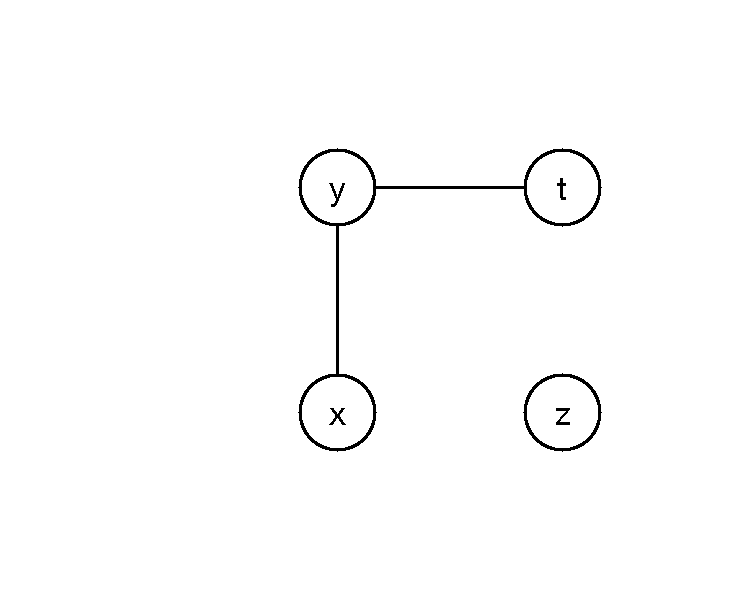
\includegraphics[height=2in]{interfere}
\end{solution}

\question[10] Given the following interference graph, assign a
register to each variable. 
\begin{center}
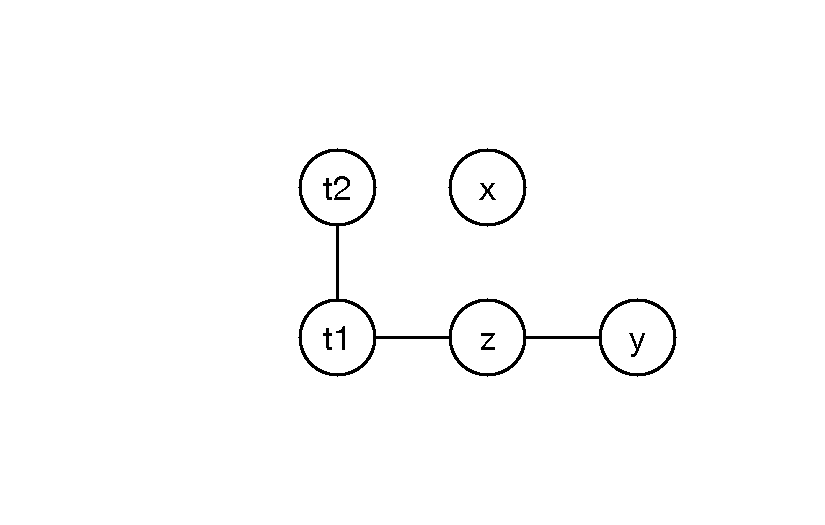
\includegraphics[height=2in]{interfere2}
\end{center}
You may use the following registers 
\begin{lstlisting}
rbx rcx rdx
\end{lstlisting}

\begin{solution}[1in]
\begin{lstlisting}
x: rbx, y: rcx, z: rbx, t1: rcx, t2: rbx
\end{lstlisting}
\end{solution}

%   Control flow and Booleans
% *   type check
% *   uncover live handling of 'if' statements
%     select instructions: eq? => cmpq, sete, movzbq
%     lower-conditionals (if (eq? a1 a2) thn els)
%     patch-instructions: cmpq, movzbq

\question[10] The following is a partial impelmentation of the type
checker for the $R_2$ language, which include integers, Booleans,
\texttt{let}, conditionals, and several primitive operations. Fill in
the match clauses for type checking \texttt{let} and \texttt{if}.

\begin{lstlisting}
   (define (typecheck-R2 env exp)
     (match exp
       [(? fixnum?) 'Integer]
       [(? boolean?) 'Boolean]
       [(? symbol?) (lookup exp env)]
       [`(program ,body)
         (let ([ty (typecheck-R2 '() body)])
           `(program (type ,ty) ,body))]
       [`(eq? ,e1 ,e2)
         (define T1 (typecheck-R2 env e1))
	 (define T2 (typecheck-R2 env e2))
	 (unless (equal? T1 T2)
           (error "eq? on different-typed values"))
	 'Boolean]
       [`(let ([,x ,exp1]) ,exp2)
         FILL ME IN
       ]
       [`(if ,cnd ,thn ,els)
         FILL ME IN
       ]
       ...
       ))
\end{lstlisting}

\begin{solution}
\begin{lstlisting}
[`(let ([,x ,exp1]) ,exp2)
  (define T1 (typecheck-R2 env exp1))
  (typecheck-R2 (cons (cons x T1) env) exp2)]

[`(if ,cnd ,thn ,els)
 (define Tc (typecheck-R2 env cnd))
 (define Tt (typecheck-R2 env thn))
 (define Te (typecheck-R2 env els))
 (unless (equal? Tc 'Boolean)
   (error "expected conditional to have type Boolean, not" Tc))
 (unless (equal? Tt Te)
   (error "expected branches of if to have same type" (list Tt Te)))
 Te]
\end{lstlisting}
\end{solution}

\question[10] Perform liveness analysis on the following programming,
listing the live-after set next to each instruction.

\begin{lstlisting}
(program (a b t3 t2 if4 x t5) (type Integer)

  (movq (int 1) (var a))

  (movq (int 2) (var b))

  (callq read_int)

  (movq (reg rax) (var t3))

  (if (eq? (var t3) (int 0))

    ((movq (var a) (var t2))

     (negq (var t2))

     (movq (var t2) (var if4)))

    ((movq (var b) (var if4))))

  (movq (var if4) (var x))

  (movq (var x) (var t5))

  (addq (int 10) (var t5))

  (movq (var t5) (reg rax)))
\end{lstlisting}

\begin{solution}
\begin{lstlisting}
(program (a b t3 t2 if4 x t5) (type Integer)
  (movq (int 1) (var a))            |$\{a,\itm{rax}\}$|
  (movq (int 2) (var b))            |$\{a,b,\itm{rax}\}$|
  (callq read_int)                  |$\{a,b,\itm{rax}\}$|
  (movq (reg rax) (var t3))         |$\{a,b,\itm{t3}\}$|
  (if (eq? (var t3) (int 0))
    ((movq (var a) (var t2))        |$\{\itm{t2}\}$|
     (negq (var t2))                |$\{\itm{t2}\}$|
     (movq (var t2) (var if4)))     |$\{\itm{if4}\}$|
    ((movq (var b) (var if4))))     |$\{\itm{if4}\}$|
  (movq (var if4) (var x))          |$\{x\}$|
  (movq (var x) (var t5))           |$\{\itm{t5}\}$|
  (addq (int 10) (var t5))          |$\{\itm{t5}\}$|
  (movq (var t5) (reg rax)))        |$\emptyset$|
\end{lstlisting}
\end{solution}

%   Tuples and GC
% *   vector representation
%        pointer mask, tuple length, forwarding bit
% *   Copying Collection
%     Cheney Algorithm
%     rootstack stuff
%     compilation
%        expose allocation
%        uncover call-live roots
%        select instructions: 
%          offset, collection-needed, allocate, vector-ref, vector-set!


\question[10] Draw a diagram of the heap as it would look after the
following expression is evaluated (but before the garbage collector is
invoked). Your diagram should include bit-level details of the
representation and annotations that describe the various parts.
\begin{lstlisting}
  (vector 4 (vector 7) #t)
\end{lstlisting}

\begin{solution}[4in]

\includegraphics[width=4in]{vectors}
\end{solution}

\question[10] Show the result of performing a copying collection given
the following heap.

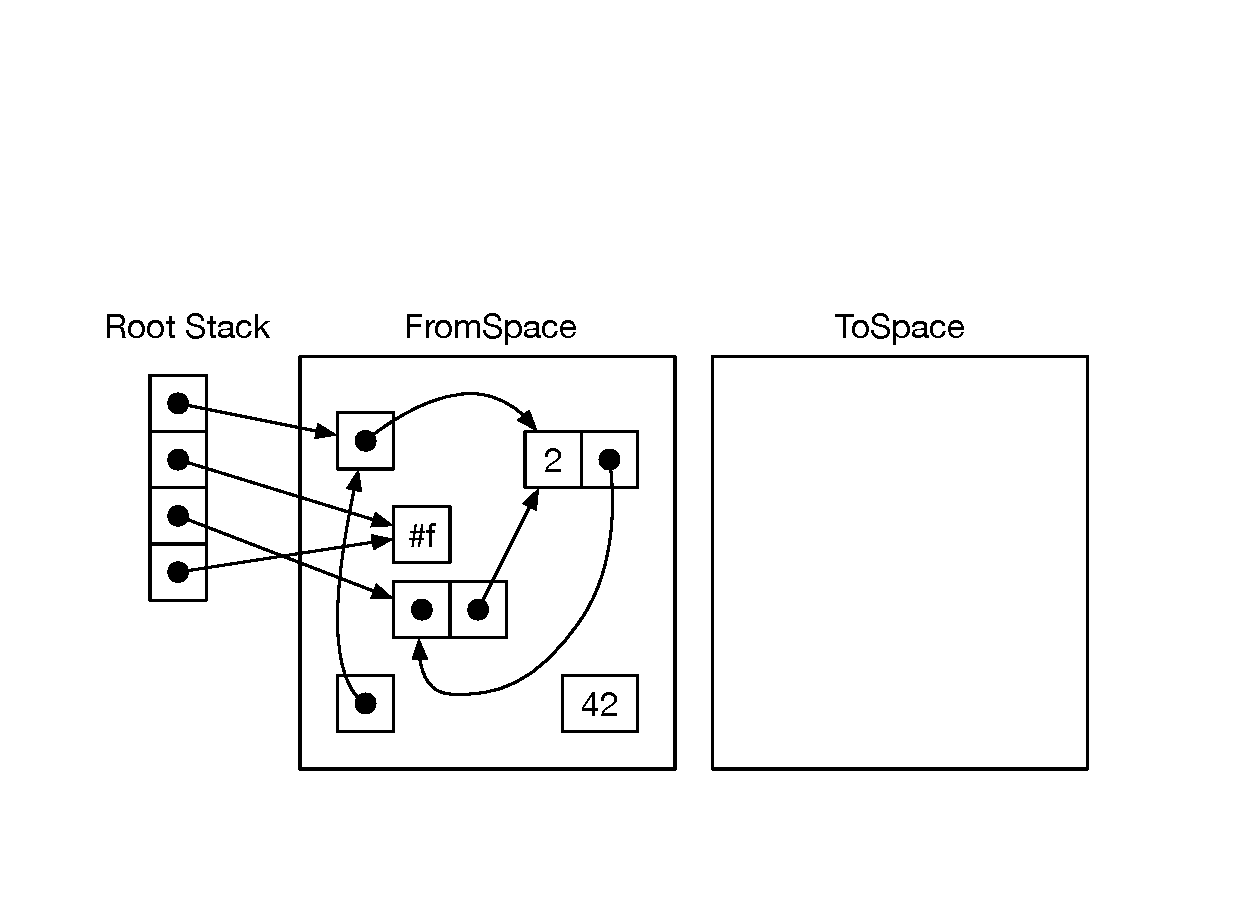
\includegraphics[width=7in]{copy-collect}


\begin{solution}

\end{solution}

\end{questions}


\end{document}
% LocalWords:  AST pyobj SSA struct def init CallFunc int fibonacci EQ LP RP 
% LocalWords:  tokenization Python's Stmt Printnl IfExp eax ebx ebp monomorphic
% LocalWords:  bool zA op expr Const InjectFrom ProjectTo GetTag stmt tmp globl
% LocalWords:  mathescape pushl movl esp subl cmpl al je sarl setne movzbl jmp
% LocalWords:  sall addl ret
